\documentclass[aspectratio=169]{beamer}

\usepackage{amsmath,amssymb}
\usepackage{graphicx}
\usepackage{tikz}
\usepackage{listings}
\usetikzlibrary{positioning,calc,arrows.meta,fit}

% =========================
% Colors
% =========================
\definecolor{PKUDarkPurple}{RGB}{63,63,191}
\definecolor{PKULightPurple}{RGB}{170,170,225}
\definecolor{PKUGrayBg}{RGB}{255,255,255}
\definecolor{PKUTextBlue}{RGB}{45,45,190}
\definecolor{CodeGray}{RGB}{245,245,245}
\definecolor{dkgreen}{rgb}{0,0.5,0}
\definecolor{gray}{rgb}{0.4,0.4,0.4}
\definecolor{mauve}{rgb}{0.58,0,0.82}

% =========================
% Global style
% =========================
\setbeamercolor{background canvas}{bg=PKUGrayBg}
\setbeamercolor{normal text}{fg=black,bg=PKUGrayBg}
\setbeamercolor{frametitle}{fg=PKUTextBlue,bg=PKUGrayBg}

\setbeamerfont{normal text}{size=\fontsize{15pt}{18pt}\selectfont}
\setbeamerfont{frametitle}{size=\fontsize{15pt}{19pt}\selectfont,series=\bfseries}
\setbeamerfont{itemize/enumerate body}{size=\fontsize{12pt}{15pt}\selectfont}
\setbeamerfont{itemize/enumerate subbody}{size=\fontsize{11pt}{14pt}\selectfont}
\setbeamerfont{footline}{size=\fontsize{10pt}{12pt}\selectfont}

\setbeamercolor{itemize item}{fg=PKUDarkPurple}
\setbeamertemplate{navigation symbols}{}
\setbeamertemplate{items}[ball]

\setbeamertemplate{headline}{}
\setbeamertemplate{footline}{}

% =========================
% Code style
% =========================
\lstset{
  basicstyle=\ttfamily\footnotesize,
  backgroundcolor=\color{CodeGray},
  keywordstyle=\color{blue},
  commentstyle=\color{dkgreen},
  stringstyle=\color{mauve},
  showstringspaces=false,
  breaklines=true,
  frame=single,
  columns=fullflexible
}

% =========================
% Custom headline
% =========================
\newcommand{\makecustomheadline}{
\begin{tikzpicture}[remember picture,overlay]
    \fill[PKUDarkPurple]
        (current page.north west)
        rectangle
        ([xshift=.50\paperwidth,yshift=-0.35cm]current page.north west);

    \fill[PKULightPurple]
        ([xshift=.50\paperwidth]current page.north west)
        rectangle
        ([xshift=\paperwidth,yshift=-0.35cm]current page.north west);
\end{tikzpicture}
}

% =========================
% Custom footline
% =========================
\newcommand{\makecustomfootline}{
\begin{tikzpicture}[remember picture,overlay]
    \fill[PKUDarkPurple]
        (current page.south west)
        rectangle
        ([xshift=.33\paperwidth,yshift=0.42cm]current page.south west);

    \fill[PKULightPurple]
        ([xshift=.33\paperwidth]current page.south west)
        rectangle
        ([xshift=.67\paperwidth,yshift=0.42cm]current page.south west);

    \fill[PKULightPurple]
        ([xshift=.67\paperwidth]current page.south west)
        rectangle
        ([xshift=\paperwidth,yshift=0.42cm]current page.south west);

    \node[anchor=center, text=white, font=\small]
        at ([xshift=.165\paperwidth,yshift=0.21cm]current page.south west)
        {\textrm{huangxun@pku.edu.cn}};

    \node[anchor=center, text=white, font=\small]
        at ([xshift=.50\paperwidth,yshift=0.21cm]current page.south west)
        {AI Enabled Control Engineering};

    \node[anchor=center, text=black, font=\small]
        at ([xshift=.83\paperwidth,yshift=0.21cm]current page.south west)
        {2026 Summer};

    \node[anchor=center, text=black, font=\small]
        at ([xshift=.965\paperwidth,yshift=0.21cm]current page.south west)
        {\insertframenumber/\inserttotalframenumber};
\end{tikzpicture}
}

\addtobeamertemplate{background}{\makecustomheadline\makecustomfootline}{}

% =========================
% Helpers
% =========================
\newcommand{\placeholderfig}[2]{
\begin{center}
\begin{tikzpicture}
    \draw[thick, rounded corners=4pt] (0,0) rectangle (8,#2);
    \node[align=center] at (4,{#2/2}) {\Large Placeholder Figure\\[3pt]\normalsize #1};
\end{tikzpicture}
\end{center}
}

\newcommand{\smallblue}[1]{\textcolor{PKUTextBlue}{#1}}

% =========================
% Title info
% =========================
\title{\textcolor{PKUTextBlue}{AI Enabled Control Engineering}}
\author{\textcolor{blue}{Professor Xun Huang}}
\institute{
Aeronautics and Astronautics\\
College of Engineering\\
Peking University\\[0.25cm]
huangxun@pku.edu.cn\\
https://xunger99.github.io/xunger/
}
\date{}

\setbeamertemplate{title page}{
    \vspace{1.0cm}
    \begin{center}
        {\fontsize{18}{22}\selectfont\bfseries \inserttitle\par}
        \vspace{0.3cm}
        {\fontsize{15}{18}\selectfont Lecture 7: Hardware Assembly, Sensor Test, and the Bellman-to-Control Bridge\par}
          \vspace{0.3cm}
        {\fontsize{15}{18}\selectfont \insertauthor\par}
        \vspace{0.15cm}
        {\fontsize{11}{13}\selectfont TA: Zhixiang Ju \quad Haozhe Wang\par}
        \vspace{0.4cm}
        {\fontsize{8}{11}\selectfont \insertinstitute\par}
    \end{center}
}

\begin{document}

% ---------------------------------
\begin{frame}
\titlepage
\end{frame}

% ---------------------------------
\begin{frame}{Recap: from Lecture 6 to Lecture 7}
\begin{itemize}
    \item Lecture 6 introduced the rotary inverted pendulum hardware modules.
    \vspace{0.25cm}
    \item We discussed the DC motor, TB6612 driver, sensors, and STM32F446RE board.
    \vspace{0.25cm}
    \item We derived the modelling objective: input $u$ determines $\theta,\dot\theta,\alpha,\dot\alpha$.
    \vspace{0.25cm}
    \item Today we connect the physical system to real sensor readings and optimal control ideas.
\end{itemize}
\end{frame}

% ---------------------------------
\begin{frame}{Lecture 7}
\begin{itemize}
    \item Build the real rotary inverted pendulum circuit .
    \vspace{0.28cm}
    \item Flash firmware and test potentiometer and encoder readings.
    \vspace{0.28cm}
    \item Start from Bellman's optimality principle and reach HJB, LQR, MPC, and RL.
\end{itemize}
\end{frame}

% ---------------------------------
\begin{frame}{Learning objectives}
By the end of this lab, students should be able to:
\vspace{0.25cm}
\begin{itemize}
    \item explain the signal flow from sensor to STM32 ;
    \vspace{0.2cm}
    \item safely wire and test the STM32--TB6612--sensor system;
    \vspace{0.2cm}
    \item convert raw potentiometer and encoder signals into angle-related measurements;
    \vspace{0.2cm}
    \item describe why LQR, MPC, and RL can be viewed under a common optimal-control framework.
\end{itemize}
\end{frame}

% ---------------------------------
\begin{frame}{Lab safety}
\begin{itemize}
    \item Do not connect the motor power before the wiring is checked.
    \vspace{0.25cm}
    \item Always connect a common ground between STM32, TB6612, and power supply.
    \vspace{0.25cm}
    \item Keep the pendulum free from obstacles before any motor test.
    \vspace{0.25cm}
    \item In this lecture, the motor is not used for closed-loop balancing yet.
    \vspace{0.25cm}
    \item When uncertain, disconnect motor power first, then debug the code.
\end{itemize}
\end{frame}

\begin{frame}{Hardware architecture}

\begin{center}
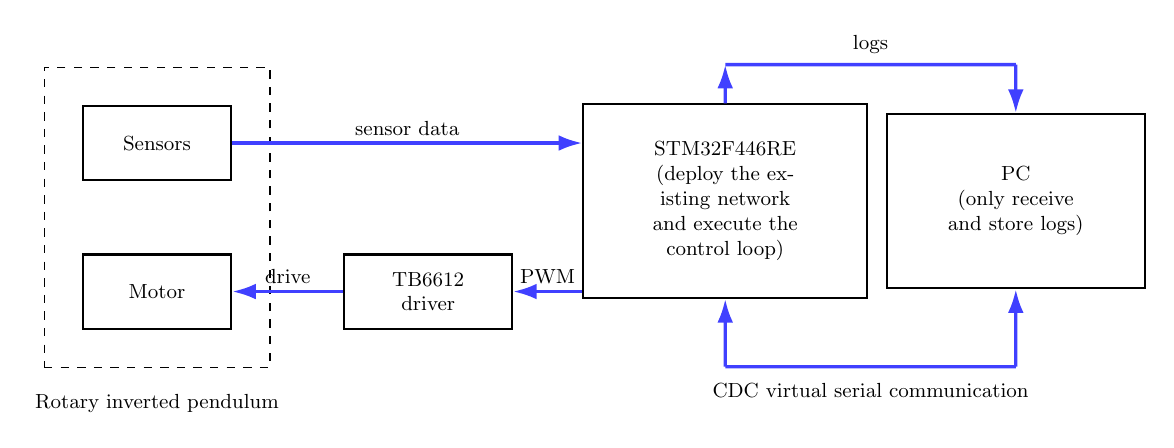
\begin{tikzpicture}[
    scale=0.82,
    transform shape,
    font=\small,
    >={Latex[length=3mm,width=2mm]},
    bluearrow/.style={->, draw=blue!75, very thick},
    blueplain/.style={-, draw=blue!75, very thick},
    smallbox/.style={draw, rectangle, thick, minimum width=2.3cm, minimum height=1.15cm, align=center},
    driverbox/.style={draw, rectangle, thick, minimum width=2.6cm, minimum height=1.15cm, align=center},
    stmbox/.style={draw, rectangle, thick, minimum width=4.4cm, minimum height=3.0cm, align=center, text width=3.9cm},
    pcbox/.style={draw, rectangle, thick, minimum width=4.0cm, minimum height=2.7cm, align=center, text width=3.5cm},
    dashedgroup/.style={draw, dashed, inner sep=0.48cm}
]

% 左侧实物系统
\node[smallbox] (sensor) at (0,0.8) {Sensors};
\node[smallbox] (motor)  at (0,-1.5) {Motor};
\node[dashedgroup, fit=(sensor)(motor)] (plantbox) {};
\node[below=0.28cm of plantbox] {Rotary inverted pendulum};

% 中间驱动与控制
\node[driverbox] (driver) at (4.2,-1.5) {TB6612\\driver};
\node[stmbox]    (stm)    at (8.8,-0.1) {STM32F446RE\\
(deploy the existing network\\
and execute the control loop)};

% 右侧 PC
\node[pcbox]     (pc)     at (13.3,-0.1) {PC\\
(only receive\\
and store logs)};

% Sensors -> STM
\draw[bluearrow] (sensor.east) -- (stm.west |- sensor.east);
\node[above] at ($(sensor.east)!0.5!(stm.west |- sensor.east)$) {sensor data};

% STM -> Driver
\draw[bluearrow] (stm.west |- driver.east) -- (driver.east);
\node[above] at ($(stm.west |- driver.east)!0.5!(driver.east)$) {PWM };

% Driver -> Motor
\draw[bluearrow] (driver.west) -- (motor.east);
\node[above] at ($(driver.west)!0.5!(motor.east)$) {drive};

% STM -> PC : logs（先上，再右，再下）
\coordinate (log_up_stm) at ($(stm.north)+(0,0.60)$);
\coordinate (log_up_pc)  at ($(pc.north)+(0,0.75)$);

\draw[bluearrow] (stm.north) -- (log_up_stm);
\draw[blueplain] (log_up_stm) -- (log_up_pc);
\draw[bluearrow] (log_up_pc) -- (pc.north);

\node[above=0.05cm] at ($(log_up_stm)!0.5!(log_up_pc)$) {logs};

% CDC 底部通信线：先画一条完全水平的主线，再分别竖直到两个框
\coordinate (cdc_left)  at ($(stm.south)+(0,-1.05)$);
\coordinate (cdc_right) at ($(pc.south)+(0,-1.2)$);

\draw[blueplain] (cdc_left) -- (cdc_right);
\draw[bluearrow] (cdc_left) -- (stm.south);
\draw[bluearrow] (cdc_right) -- (pc.south);

\node[below=0.14cm] at ($(cdc_left)!0.5!(cdc_right)$) {CDC virtual serial communication};

\end{tikzpicture}
\vspace{1.3cm}
\end{center}

\end{frame}


% ---------------------------------
\begin{frame}{DC Power Jack: Interface and Pins}

\begin{columns}[T,totalwidth=\textwidth]

% ================= left column =================
\begin{column}{0.45\textwidth}


\begin{block}{Pin definition}
\begin{itemize}
    \item Pin 1: positive terminal, connected to $V_{\mathrm{in}}+$.
    \vspace{0.15cm}
    \item Pin 2: negative terminal, connected to GND.
    \vspace{0.15cm}
    \item Pin 3: switched negative terminal, not used in our circuit.
\end{itemize}
\end{block}

\vspace{0.15cm}

\begin{alertblock}{Pins used in our experiment}
\begin{center}
\Large
\textcolor{PKUDarkPurple}{1: $V_{\mathrm{in}}+(VM)$}
\qquad
\textcolor{PKUDarkPurple}{3: GND}
\end{center}
\end{alertblock}

\end{column}

% ================= right column =================
\begin{column}{0.52\textwidth}

\begin{center}
    \includegraphics[width=0.60\textwidth]{DC.png}
\end{center}

\vspace{-0.15cm}

\begin{center}
\small
DC-002 / DC-005 power jack used for external DC input.
\end{center}

\vspace{0.15cm}


\end{column}

\end{columns}

\end{frame}




% ---------------------------------
\begin{frame}{Wiring Diagram of the PC--STM32 RIP System}

\begin{center}
    \includegraphics[width=0.92\textwidth]{wire.png}
\end{center}

\vspace{-0.1cm}


\end{frame}




% ---------------------------------
\begin{frame}{TA Check Before Power-on}

\begin{center}
\Large
Before power-on, each group should ask a TA to check the circuit.
\end{center}

\vspace{0.35cm}

\begin{enumerate}
    \item Is the STM32 logic supply connected to $3.3\,\mathrm{V}$ instead of $5\,\mathrm{V}$?
    \vspace{0.3cm}

    \item Are all Dupont wires firmly connected?
    \vspace{0.3cm}

    \item Are the breadboard vertical rails correctly assigned?
    \vspace{0.3cm}

    \item Are there four wires on the GND rail and four wires on the $3.3\,\mathrm{V}$ rail?
    \vspace{0.3cm}

    \item Is the external $12\,\mathrm{V}$ supply connected only to the TB6612 motor-power side?
\end{enumerate}
\end{frame}



% ---------------------------------
\begin{frame}{Next step: flash sensor-test firmware}

\begin{itemize}
    \item The circuit has been connected and checked.
    \vspace{0.35cm}

    \item Now we flash a simple test program to STM32.
    \vspace{0.35cm}

    \item This program does not control the motor.
    \vspace{0.35cm}

    \item It only reads:
    \vspace{0.15cm}
    \begin{itemize}
        \item potentiometer raw value;
        \item encoder count value.
    \end{itemize}
\end{itemize}

\vspace{0.25cm}

\begin{alertblock}{Safety reminder}
\small
During this test, the external motor power can remain disconnected.
\end{alertblock}

\end{frame}





% ---------------------------------
% ---------------------------------


% ---------------------------------
\begin{frame}[fragile]{Step 1: create a new Arduino sketch}



\begin{lstlisting}[basicstyle=\ttfamily\tiny]
static const int PIN_POT   = A0;
static const int PIN_ENC_A = 2;
static const int PIN_ENC_B = 3;

static volatile long g_enc = 0;

void setup() {
    Serial.begin(115200);

    pinMode(PIN_POT, INPUT);

    pinMode(PIN_ENC_A, INPUT_PULLUP);
    pinMode(PIN_ENC_B, INPUT_PULLUP);

    attachInterrupt(
        digitalPinToInterrupt(PIN_ENC_A),
        isr_enc_a,
        CHANGE
    );

    attachInterrupt(
        digitalPinToInterrupt(PIN_ENC_B),
        isr_enc_b,
        CHANGE
    );
}
\end{lstlisting}

\end{frame}


% ---------------------------------
\begin{frame}[fragile]{Step 1: serial output code}

\begin{itemize}
    \item Then add the loop function below.
    \vspace{0.15cm}

    \item Save the sketch before uploading it to STM32.
\end{itemize}

\vspace{0.12cm}

\begin{lstlisting}[basicstyle=\ttfamily\tiny]
void loop() {
    int pot_raw = analogRead(PIN_POT);

    noInterrupts();
    long enc_now = g_enc;
    interrupts();

    Serial.print("pot_raw = ");
    Serial.print(pot_raw);

    Serial.print(", enc = ");
    Serial.println(enc_now);

    delay(100);
}
\end{lstlisting}

\vspace{0.12cm}

\begin{block}{Purpose}
\small
The STM32 will send potentiometer and encoder values to the PC every 100 ms.
\end{block}

\end{frame}



% ---------------------------------
\begin{frame}{Step 2: select board and port}

\begin{itemize}
    \item Connect STM32 to the PC using the onboard miniUSB cable.
    \vspace{0.35cm}

    \item In Arduino IDE, select the correct board:
    \vspace{0.15cm}
    \begin{itemize}
        \item \texttt{Nucleo-64}
        \item or the corresponding STM32F446RE board option.
    \end{itemize}
    \vspace{0.35cm}

    \item Select the correct serial port.
\end{itemize}

\vspace{0.25cm}

\begin{alertblock}{Common mistake}
\small
If the wrong board or port is selected, the code cannot be uploaded successfully.
\end{alertblock}

\end{frame}

% ---------------------------------
\begin{frame}{Step 3: upload the firmware}

\begin{itemize}
    \item Click the \textbf{Upload} button in Arduino IDE.
    \vspace{0.35cm}

    \item Wait until the IDE shows that uploading is completed.
    \vspace{0.35cm}

    \item If uploading fails:
    \vspace{0.15cm}
    \begin{itemize}
        \item check the USB cable;
        \item check the board selection;
        \item check the serial port;
        \item reconnect STM32 and try again.
    \end{itemize}
\end{itemize}

\vspace{0.25cm}

\begin{block}{Expected result}
\small
After successful upload, STM32 starts reading the sensors automatically.
\end{block}

\end{frame}

% ---------------------------------
\begin{frame}{Step 4: open the serial monitor}

\begin{itemize}
    \item After uploading, open:
    \vspace{0.15cm}
    \begin{center}
    \texttt{Tools} $\rightarrow$ \texttt{Serial Monitor}
    \end{center}
    \vspace{0.25cm}

    \item Set the baud rate to:
    \vspace{0.15cm}
    \begin{center}
    \Large
    \textcolor{PKUDarkPurple}{115200}
    \end{center}
    \vspace{0.25cm}

    \item The serial monitor should display sensor data continuously.
\end{itemize}

\vspace{0.2cm}

\begin{alertblock}{Important}
\small
The baud rate in the serial monitor must match the baud rate in the firmware.
\end{alertblock}

\end{frame}

% ---------------------------------
\begin{frame}[fragile]{Expected serial output}

\begin{itemize}
    \item If the firmware is running correctly, the serial monitor shows values like:
\end{itemize}

\vspace{0.2cm}

\begin{lstlisting}
pot_raw = 3092, enc = 10000
pot_raw = 3091, enc = 10002
pot_raw = 3093, enc = 10005
\end{lstlisting}

\vspace{0.2cm}

\begin{itemize}
    \item \texttt{pot\_raw}: raw ADC value of the potentiometer.
    \vspace{0.2cm}

    \item \texttt{enc}: accumulated encoder count.
\end{itemize}

\vspace{0.2cm}

\begin{block}{What students should do}
\small
Rotate the pendulum and rotary arm by hand, then observe how the two values change.
\end{block}

\end{frame}

% ---------------------------------
\begin{frame}{From raw sensor values to angles}

\begin{itemize}
    \item In the previous firmware, we printed raw values:
    \vspace{0.25cm}

    \begin{center}
    \texttt{pot\_raw}  \qquad \texttt{enc}
    \end{center}

    \vspace{0.25cm}

    \item Now we make a minimum modification:
    \vspace{0.15cm}
    \begin{itemize}
        \item convert encoder count to arm angle $\theta$;
        \item convert potentiometer raw value to pendulum angle $\alpha$.
    \end{itemize}

    \vspace{0.25cm}

    \item This conversion method will be used as the common firmware convention in later experiments.
\end{itemize}

\vspace{0.25cm}


\end{frame}

% ---------------------------------
\begin{frame}{Sensor logging files provided}

\begin{itemize}
    \item We provide two files for this experiment:
    \vspace{0.25cm}

    \begin{center}
    \texttt{rip\_sensor\_logger.ino}
    \qquad
    \texttt{rip\_record\_10s.py}
    \end{center}

    \vspace{0.25cm}

    \item The STM32 firmware reads the potentiometer and encoder at 200 Hz.
    \vspace{0.25cm}

    \item The Python script sends the \texttt{GO} command, records data for 10 s,
    saves a CSV file, and plots the angle curves.
\end{itemize}

\vspace{0.25cm}

\begin{alertblock}{Important}
\small
The motor is not controlled in this test. This step is only for sensor calibration and data logging.
\end{alertblock}

\end{frame}


% ---------------------------------
\begin{frame}{Step 1: calibrate the potentiometer zero}

\begin{enumerate}
    \item Hold the vertical pendulum arm at the upright position.
    \vspace{0.3cm}

    \item Keep the pendulum still.
    \vspace{0.3cm}

    \item Open the Arduino Serial Monitor.
    \vspace{0.3cm}

    \item Read the current potentiometer raw value.
    \vspace{0.3cm}

    \item Modify \texttt{POT\_ZERO} in \texttt{rip\_sensor\_logger.ino}.
\end{enumerate}

\vspace{0.25cm}

\begin{block}{Example}
\small
If the serial monitor shows \texttt{RAW,pot=3132,...}, then set:
\texttt{POT\_ZERO = 3132}.
\end{block}

\end{frame}


% ---------------------------------
\begin{frame}[fragile]{Step 2: modify the calibration constants}

\begin{lstlisting}[basicstyle=\ttfamily\small]
static volatile int32_t POT_ZERO = 3132;
static volatile int32_t POT_DOWN_RAW = 1036;
\end{lstlisting}

\vspace{0.3cm}

\begin{itemize}
    \item \texttt{POT\_ZERO}: raw value when the pendulum is upright.
    \vspace{0.25cm}

    \item \texttt{POT\_DOWN\_RAW}: raw value when the pendulum is naturally hanging down.
    \vspace{0.25cm}

    \item After modifying these values, upload the firmware again.
\end{itemize}

\vspace{0.2cm}

\begin{alertblock}{Very important}
\small
A wrong \texttt{POT\_ZERO} will cause a wrong pendulum angle $\alpha$.
This will directly affect all later control experiments.
\end{alertblock}

\end{frame}


% ---------------------------------
\begin{frame}{Step 3: upload the firmware}

\begin{itemize}
    \item Open \texttt{rip\_sensor\_logger.ino} in Arduino IDE.
    \vspace{0.3cm}

    \item Select the correct STM32 board and serial port.
    \vspace{0.3cm}

    \item Upload the firmware to STM32.
    \vspace{0.3cm}

    \item Open the Serial Monitor and set the baud rate to:
\end{itemize}

\vspace{0.15cm}

\begin{center}
\Large
\textcolor{PKUDarkPurple}{921600}
\end{center}

\vspace{0.15cm}

\begin{block}{Expected before \texttt{GO}}
\small
The STM32 prints raw sensor readings slowly, so students can check the potentiometer and encoder values.
\end{block}

\end{frame}


% ---------------------------------
\begin{frame}{Step 4: run the Python logging script}

\begin{itemize}
    \item Close the Arduino Serial Monitor first.
    \vspace{0.3cm}

    \item Open a terminal in the folder containing \texttt{rip\_record\_10s.py}.
    \vspace{0.3cm}

    \item Run:
\end{itemize}

\vspace{0.1cm}

\begin{center}
\texttt{python rip\_record\_10s.py}
\end{center}

\vspace{0.25cm}

\begin{itemize}
    \item The script automatically finds the serial port when possible.
    \vspace{0.25cm}

    \item It sends \texttt{GO} to STM32 and records data for 10 s.
\end{itemize}

\end{frame}


% ---------------------------------
\begin{frame}{Step 5: what happens after \texttt{GO}}

\begin{itemize}
    \item STM32 records the current encoder count as the zero position:
    \vspace{0.15cm}

    \begin{center}
    current arm position $\Rightarrow \theta = 0$
    \end{center}

    \vspace{0.25cm}

    \item STM32 sends one data line every $5\,\mathrm{ms}$.
    \vspace{0.25cm}

    \item The serial output format is:
\end{itemize}

\vspace{0.15cm}

\begin{center}
\small
\texttt{DATA,t\_ms,pot,enc,theta,alpha,theta\_dot,alpha\_dot}
\end{center}

\vspace{0.25cm}

\begin{block}{After 10 seconds}
\small
Python saves the latest CSV file and automatically plots angle and angular-velocity curves.
\end{block}

\end{frame}


% ---------------------------------
\begin{frame}{Expected output}

\begin{itemize}
    \item A CSV file will be generated:
    \vspace{0.15cm}

    \begin{center}
    \texttt{rip\_sensor\_log\_YYYYMMDD\_HHMMSS.csv}
    \end{center}

    \vspace{0.25cm}

    \item A figure will also be generated:
    \vspace{0.15cm}

    \begin{center}
    \texttt{rip\_sensor\_log\_YYYYMMDD\_HHMMSS.png}
    \end{center}

    \vspace{0.25cm}

    \item The figure contains:
    \vspace{0.15cm}
    \begin{itemize}
        \item $\theta(t)$ and $\alpha(t)$;
        \item $\dot\theta(t)$ and $\dot\alpha(t)$.
    \end{itemize}
\end{itemize}

\end{frame}

% ---------------------------------
\begin{frame}{Motor test files provided}

\begin{itemize}
    \item We now test whether STM32 can drive the motor through TB6612FNG.
    \vspace{0.25cm}

    \item We provide two files:
    \vspace{0.15cm}

    \begin{center}
    \texttt{rip\_motor\_test.ino}
    \qquad
    \texttt{rip\_motor\_test\_10s.py}
    \end{center}

    \vspace{0.25cm}

    \item The new firmware is based on the previous sensor logger.
    \vspace{0.25cm}

    \item It keeps 200 Hz sensor logging and adds a safe PWM motor test.
\end{itemize}

\vspace{0.2cm}

\begin{alertblock}{Before motor test}
\small
Make sure the pendulum is free to move, all wires are firm, and the external 12 V motor power is connected only to the TB6612 motor-power side.
\end{alertblock}

\end{frame}


% ---------------------------------
\begin{frame}{Run the motor test}

\begin{enumerate}
    \item Upload \texttt{rip\_motor\_test.ino} to STM32.
    \vspace{0.25cm}

    \item Close the Arduino Serial Monitor.
    \vspace{0.25cm}

    \item Run the Python script:
    \vspace{0.1cm}

    \begin{center}
    \texttt{python rip\_motor\_test\_10s.py}
    \end{center}

    \vspace{0.2cm}

    \item The Python script sends \texttt{GO} and then sends a small PWM test sequence.
    \vspace{0.25cm}

    \item After 10 s, it saves a CSV file and plots the sensor and PWM curves.
\end{enumerate}

\vspace{0.2cm}

\begin{block}{Expected result}
\small
The motor should rotate gently according to the PWM command, while the PC records
$\theta$, $\alpha$, $\dot{\theta}$, $\dot{\alpha}$, and PWM.
\end{block}

\end{frame}









% ---------------------------------
\begin{frame}{Bellman, optimal control, and reinforcement learning}

\begin{itemize}
    \item We have just built and tested the real rotary inverted pendulum system.
    \vspace{0.25cm}

    \item Now we return to the central question:
    \vspace{0.15cm}
    \begin{center}
    \Large
    \textcolor{PKUDarkPurple}{How should a controller choose the best action?}
    \end{center}

    \vspace{0.2cm}

    \item This question leads to Bellman's optimality principle.
    \vspace{0.25cm}

    \item From this principle, we can understand LQR, MPC, and DQN under one framework.
\end{itemize}

\vspace{0.2cm}

\begin{block}{Key message}
\small
AI-based control is not isolated from classical control. 
It can be viewed as approximate optimal control when the model, value function, or action space becomes difficult to handle explicitly.
\end{block}

\end{frame}


% ---------------------------------
\begin{frame}{Unified view under Bellman's optimality principle}

\begin{center}
\resizebox{0.94\textwidth}{!}{
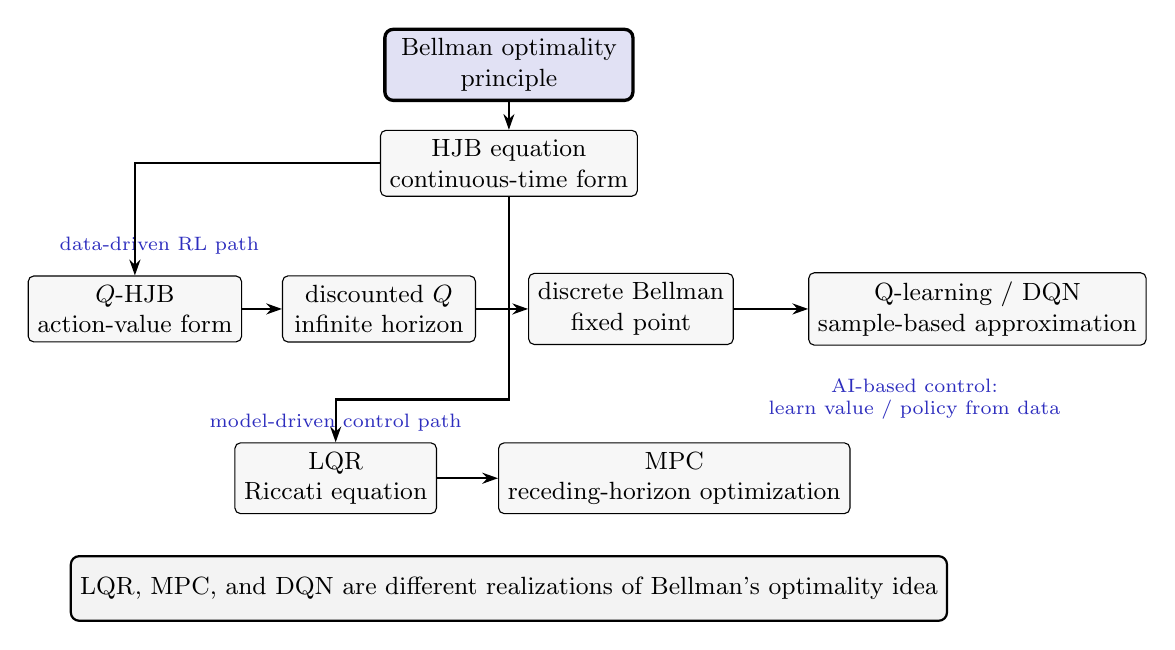
\begin{tikzpicture}[
    font=\small,
    box/.style={
        rectangle,
        rounded corners=2pt,
        draw=black,
        align=center,
        minimum height=0.78cm,
        minimum width=2.45cm,
        fill=gray!5
    },
    main/.style={
        rectangle,
        rounded corners=3pt,
        draw=black,
        very thick,
        align=center,
        minimum height=0.82cm,
        minimum width=3.15cm,
        fill=PKULightPurple!35
    },
    final/.style={
        rectangle,
        rounded corners=3pt,
        draw=black,
        thick,
        align=center,
        minimum height=0.82cm,
        minimum width=9.8cm,
        fill=gray!8
    },
    arrow/.style={
        -{Stealth[length=2mm,width=1.4mm]},
        thick
    },
    pathlabel/.style={
        font=\scriptsize,
        align=center,
        text=PKUTextBlue
    }
]

\node[main] (bellman) at (0,0) {Bellman optimality\\principle};
\node[box]  (hjb)     at (0,-1.25) {HJB equation\\continuous-time form};

\node[pathlabel, anchor=east] at (-3.05,-2.30) {data-driven RL path};

\node[box] (qhjb)      at (-4.75,-3.10) {$Q$-HJB\\action-value form};
\node[box] (discount)  at (-1.65,-3.10) {discounted $Q$\\infinite horizon};
\node[box] (dbellman)  at (1.55,-3.10) {discrete Bellman\\fixed point};
\node[box, minimum width=2.80cm] (dqn) at (5.95,-3.10) {Q-learning / DQN\\sample-based approximation};

\node[pathlabel] at (-2.20,-4.55) {model-driven control path};

\node[box] (lqr) at (-2.20,-5.25) {LQR\\Riccati equation};
\node[box, minimum width=2.85cm] (mpc) at (2.10,-5.25) {MPC\\receding-horizon optimization};

\node[final] (summary) at (0,-6.65)
{LQR, MPC, and DQN are different realizations of Bellman's optimality idea};

\draw[arrow] (bellman.south) -- (hjb.north);

\draw[arrow]
    (hjb.west) -- (-4.75,-1.25)
    -- (-4.75,-2.45)
    -- (qhjb.north);

\draw[arrow]
    (hjb.south) -- (0,-4.25)
    -- (-2.20,-4.25)
    -- (lqr.north);

\draw[arrow] (qhjb.east) -- (discount.west);
\draw[arrow] (discount.east) -- (dbellman.west);
\draw[arrow] (dbellman.east) -- (dqn.west);

\draw[arrow] (lqr.east) -- (mpc.west);



\node[align=center, font=\scriptsize, text=PKUTextBlue] at (5.15,-4.25)
{AI-based control:\\learn value / policy from data};

\end{tikzpicture}
}
\end{center}

\end{frame}


% ---------------------------------
\begin{frame}{Bellman's optimality principle}

\begin{itemize}
    \item A globally optimal policy has a recursive structure.
    \vspace{0.3cm}

    \item After the first action is chosen, the remaining policy must still be optimal for the new state.
    \vspace{0.3cm}

    \item Therefore, an optimal control problem can be decomposed into:
    \vspace{0.15cm}
    \begin{center}
    \textcolor{PKUDarkPurple}{current cost}
    \quad $+$ \quad
    \textcolor{PKUDarkPurple}{optimal future cost}.
    \end{center}
\end{itemize}

\vspace{0.25cm}

\begin{block}{Intuition}
\small
The best current action should not only reduce the immediate cost, but also put the system into a state with small future cost.
\end{block}

\end{frame}


% ---------------------------------
\begin{frame}{Continuous-time optimal control problem}

Consider a deterministic continuous-time system:
\[
\dot{x}(t)=f(x(t),u(t),t),
\qquad
x(t)\in\mathbb{R}^n,\quad u(t)\in\mathcal U .
\]

\vspace{0.25cm}

The finite-horizon cost is:
\[
J(u(\cdot);x_0)
=
\int_0^T g(x(t),u(t),t)\,dt+h(x(T)).
\]

\vspace{0.25cm}

The optimal cost-to-go is:
\[
J^*(t,x)
=
\inf_{u(\cdot)}
\left\{
\int_t^T g(x(s),u(s),s)\,ds+h(x(T))
\right\}.
\]

\vspace{0.15cm}


$J^*(t,x)$ measures the minimum remaining cost from state $x$ at time $t$.


\end{frame}

% ---------------------------------
\begin{frame}{Discrete cost and Bellman recursion}

Using a small time step $\delta$, define
\[
t_k=k\delta,\qquad x_k=x(t_k),\qquad u_k=u(t_k).
\]

The continuous dynamics can be approximated by
\[
x_{k+1}
\approx
x_k+f(x_k,u_k,t_k)\delta .
\]

\vspace{0.1cm}

The finite-horizon cost becomes
\[
\tilde J(\{u_k\};x_0)
=
h(x_N)
+
\sum_{k=0}^{N-1}
g(x_k,u_k,t_k)\delta .
\]

\vspace{0.1cm}

Therefore, the optimal cost-to-go satisfies
\[
\tilde{J}^*(t_k,x)
=
\min_{u\in\mathcal U}
\left\{
g(x,u,t_k)\delta
+
\tilde{J}^*
\bigl(t_{k+1},x+f(x,u,t_k)\delta\bigr)
\right\}.
\]

\vspace{0.1cm}



\end{frame}

% ---------------------------------
% ---------------------------------
\begin{frame}{From Bellman recursion to HJB}

From the previous slide, Bellman recursion gives
\[
\tilde{J}^*(k\delta,x)
=
\min_{u\in\mathcal U}
\left\{
g(x,u,k\delta)\delta
+
\tilde{J}^*
\bigl((k+1)\delta,\,
x+f(x,u,k\delta)\delta\bigr)
\right\}.
\]

\vspace{0.15cm}

Assume \(\tilde{J}^*(t,x)\) is sufficiently smooth. Then
\[
\begin{aligned}
&\tilde{J}^*
\bigl((k+1)\delta,\,
x+f(x,u,k\delta)\delta\bigr) \\
&=
\tilde{J}^*(k\delta,x)
+
\frac{\partial \tilde{J}^*}{\partial t}(k\delta,x)\delta
+
\nabla_x\tilde{J}^*(k\delta,x)^\top
f(x,u,k\delta)\delta
+
o(\delta).
\end{aligned}
\]

\vspace{0.1cm}

Substitute the Taylor expansion into Bellman recursion and cancel
\(\tilde{J}^*(k\delta,x)\).

\end{frame}

% ---------------------------------
\begin{frame}{From Bellman recursion to HJB}

After substitution and cancellation,
\[
0
=
\min_{u\in\mathcal U}
\left\{
\left[
g(x,u,k\delta)
+
\frac{\partial \tilde{J}^*}{\partial t}(k\delta,x)
+
\nabla_x\tilde{J}^*(k\delta,x)^\top
f(x,u,k\delta)
\right]\delta
+
o(\delta)
\right\}.
\]

\vspace{0.15cm}

Dividing by \(\delta\), and letting
\[
\delta\to0,
\qquad
k\delta\to t,
\]
we obtain
\[
0
=
\min_{u\in\mathcal U}
\left\{
g(x,u,t)
+
\frac{\partial J^*}{\partial t}(t,x)
+
\nabla_xJ^*(t,x)^\top f(x,u,t)
\right\}.
\]

\end{frame}
% ---------------------------------
\begin{frame}{From Bellman recursion to HJB}

\[
-\frac{\partial J^*}{\partial t}
=
\min_{u\in\mathcal U}
\left\{
g(x,u,t)+\nabla_xJ^*(t,x)^\top f(x,u,t)
\right\}.
\]

\vspace{0.25cm}

\begin{itemize}
    \item $g(x,u,t)$: immediate cost.
    \vspace{0.25cm}

    \item $\nabla_xJ^*{}^\top f$: effect of the current action on future cost.
    \vspace{0.25cm}

    \item The optimal action minimizes the sum of these two terms.
\end{itemize}

\vspace{0.25cm}

\begin{alertblock}{Difficulty}
\small
For nonlinear high-dimensional systems, HJB is usually a nonlinear partial differential equation and is hard to solve directly.
\end{alertblock}

\end{frame}


% ---------------------------------
\begin{frame}{LQR: a special solvable case of HJB}

For a linear system:
\[
\dot{x}=Ax+Bu,
\]

with quadratic cost:
\[
J
=
\frac12 x(T)^\top Hx(T)
+
\frac12
\int_t^T
\left(
x^\top R_{xx}x
+
u^\top R_{uu}u
\right)d\tau .
\]

\vspace{0.2cm}

Because the system is linear and the cost is quadratic, assume:
\[
J^*(t,x)=\frac12 x^\top P(t)x .
\]

\vspace{0.2cm}

\begin{block}{Key idea}
\small
LQR is obtained by substituting a quadratic value function into the HJB equation.
\end{block}

\end{frame}


% ---------------------------------
\begin{frame}{From HJB to the LQR feedback law}

For
\[
J^*(t,x)=\frac12x^\top P(t)x,
\]
we have:
\[
\nabla_xJ^*(t,x)=P(t)x .
\]


Substituting into HJB:
\[
-\frac12x^\top\dot P x
=
\min_u
\left\{
\frac12x^\top R_{xx}x
+
\frac12u^\top R_{uu}u
+
x^\top P(Ax+Bu)
\right\}.
\]



Taking derivative with respect to $u$:
\[
R_{uu}u+B^\top Px=0.
\]

Therefore:
\[
u^*(t)=-R_{uu}^{-1}B^\top P(t)x(t).
\]

\end{frame}


% ---------------------------------
\begin{frame}{Riccati equation and LQR controller}

After substituting the optimal $u^*$ back into HJB:
\[
-\dot P
=
PA+A^\top P+R_{xx}
-
PBR_{uu}^{-1}B^\top P .
\]

\vspace{0.2cm}

For infinite-horizon time-invariant LQR:
\[
A^\top P+PA+R_{xx}
-
PBR_{uu}^{-1}B^\top P=0.
\]

\vspace{0.2cm}

The feedback controller is:
\[
u=-Kx,
\qquad
K=R_{uu}^{-1}B^\top P.
\]

\vspace{0.2cm}

\begin{block}{Conclusion}
\small
LQR is Bellman's optimality principle under linear dynamics, quadratic cost, and a quadratic value-function assumption.
\end{block}

\end{frame}


% ---------------------------------
\begin{frame}{MPC: another model-driven realization}

HJB gives the optimal feedback law if $J^*$ is known:
\[
u^*(t,x)
\in
\arg\min_u
\left\{
g(x,u,t)
+
\nabla_xJ^*(t,x)^\top f(x,u,t)
\right\}.
\]

\vspace{0.25cm}

But for general systems:
\begin{itemize}
    \item the HJB equation is hard to solve;
    \vspace{0.2cm}
    \item constraints are important in real hardware;
    \vspace{0.2cm}
    \item the controller must be computable online.
\end{itemize}

\vspace{0.25cm}

\begin{block}{MPC idea}
\small
Instead of solving the full HJB equation, solve a finite-horizon optimization problem repeatedly at each sampling time.
\end{block}

\end{frame}


% ---------------------------------
\begin{frame}{MPC finite-horizon optimization}

At time step $k$, given the current state $x_k$, solve:
\[
U^*(x_k)
=
\arg\min_U
\left\{
\sum_{i=0}^{N-1}
\ell(x_{k+i|k},u_{k+i|k})
+
V_f(x_{k+N|k})
\right\}.
\]



Subject to:
\[
x_{k+i+1|k}
=
F(x_{k+i|k},u_{k+i|k}),
\qquad
x_{k|k}=x_k .
\]



The optimal control sequence is:
\[
U^*
=
\begin{bmatrix}
u^*_{k|k}&u^*_{k+1|k}&\cdots&u^*_{k+N-1|k}
\end{bmatrix}^\top .
\]



\begin{alertblock}{Receding horizon}
\small
Only the first control input $u^*_{k|k}$ is applied. Then the state is measured again and the optimization is solved again.
\end{alertblock}

\end{frame}


% ---------------------------------
\begin{frame}{LQR and MPC under the Bellman viewpoint}

\begin{center}
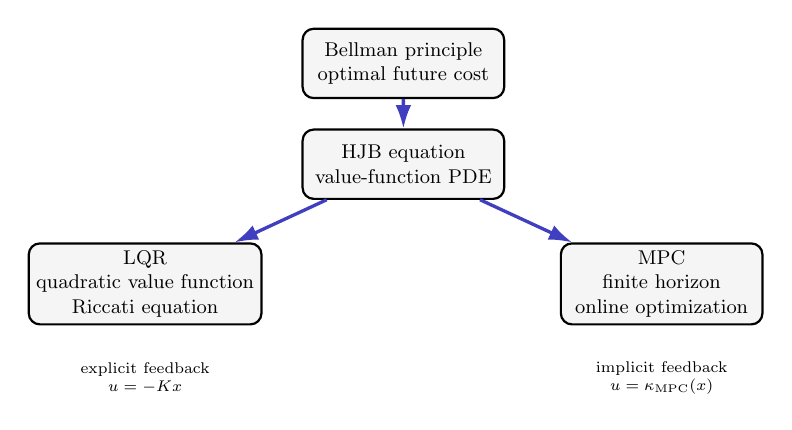
\begin{tikzpicture}[
    scale=0.80,
    transform shape,
    font=\small,
    box/.style={
        draw,
        rounded corners=4pt,
        thick,
        align=center,
        minimum width=3.2cm,
        minimum height=1.1cm,
        fill=CodeGray
    },
    arrow/.style={-{Latex[length=3mm,width=2mm]}, very thick, draw=PKUDarkPurple}
]

\node[box] (bellman) at (0,2.0) {Bellman principle\\optimal future cost};
\node[box] (hjb) at (0,0.4) {HJB equation\\value-function PDE};

\node[box] (lqr) at (-4.1,-1.5) {LQR\\quadratic value function\\Riccati equation};

\node[box] (mpc) at (4.1,-1.5) {MPC\\finite horizon\\online optimization};

\draw[arrow] (bellman) -- (hjb);
\draw[arrow] (hjb) -- (lqr);
\draw[arrow] (hjb) -- (mpc);

\node[align=center, font=\scriptsize] at (-4.1,-3.0)
{explicit feedback\\$u=-Kx$};

\node[align=center, font=\scriptsize] at (4.1,-3.0)
{implicit feedback\\$u=\kappa_{\mathrm{MPC}}(x)$};

\end{tikzpicture}
\end{center}



\begin{block}{For the rotary inverted pendulum}
\small
LQR is fast and simple near the upright equilibrium. 
MPC can include input constraints and prediction, but requires more online computation.
\end{block}

\end{frame}


% ---------------------------------
\begin{frame}{Why introduce the $Q$ function?}

HJB selects the optimal action by:
\[
u^*(t,x)
\in
\arg\min_u
\left\{
g(x,u,t)
+
\nabla_xJ^*(t,x)^\top f(x,u,t)
\right\}.
\]


This expression depends on:
\begin{itemize}
    \item the system model $f(x,u,t)$;
    \vspace{0.2cm}
    \item the value-function gradient $\nabla_xJ^*$;
    \vspace{0.2cm}
    \item solving or approximating the HJB equation.
\end{itemize}


\begin{block}{Action-value idea}
\small
Instead of evaluating only states, define a value for each state-action pair:
\[
Q(x,u).
\]
Then action selection can be written as
\[
u^*(x)\in\arg\min_u Q(x,u).
\]
\end{block}

\end{frame}

% ---------------------------------
\begin{frame}{Continuous-time action-value function}

To define an action-value function in continuous time, we treat the current control value \(u\) as part of the state.

\vspace{0.15cm}

Introduce an augmented system:
\[
\begin{cases}
\dot{x}(t)=f(x(t),u(t),t),\\
\dot{u}(t)=a(t),
\end{cases}
\qquad
u(t)\in\mathcal U,\quad \|a(t)\|_2\le M .
\]

\vspace{0.15cm}

Here \(a(t)\) is the rate of change of the control input.

\vspace{0.2cm}

\begin{block}{Why introduce \(a(t)\)?}
\small
In continuous time, the current action \(u\) is not just selected once and then forgotten.
To define \(Q(x,u,t)\), we fix the current value of \(u\), and optimize how \(u\) changes afterwards.
\end{block}

\end{frame}


% ---------------------------------
\begin{frame}{Definition of continuous-time \(Q\) function}

Given current state \(x\), current control value \(u\), and time \(t\), define
\[
\begin{aligned}
Q(x,u,t)
\triangleq
\inf_{a(\cdot)}
\Bigg\{
&\int_t^T g(x(s),u(s),s)\,ds+h(x(T))
\\
&\left|
\begin{array}{l}
\dot{x}(s)=f(x(s),u(s),s),\\
\dot{u}(s)=a(s),\\
x(t)=x,\quad u(t)=u,\\
u(s)\in\mathcal U,\quad \|a(s)\|_2\le M
\end{array}
\right.
\Bigg\}.
\end{aligned}
\]

\vspace{0.15cm}

\begin{block}{Relation between \(J^*\) and \(Q\)}
\[
J^*(t,x)=\min_{u\in\mathcal U}Q(x,u,t).
\]
\small
The optimal state value is obtained by choosing the best initial control value \(u\).
\end{block}

\end{frame}


% ---------------------------------
\begin{frame}{Dynamic programming equation for \(Q\)}

For any small time interval \(h>0\), Bellman's principle gives
\[
Q(x,u,t)
=
\inf_{\|a(\cdot)\|_2\le M}
\left\{
\int_t^{t+h}g(x(s),u(s),s)\,ds
+
Q(x(t+h),u(t+h),t+h)
\right\}.
\]

\vspace{0.2cm}

The terminal state \((x(t+h),u(t+h))\) is generated by
\[
\dot{x}=f(x,u,t),
\qquad
\dot{u}=a .
\]

\vspace{0.2cm}

\begin{block}{One-step structure}
\small
Current \(Q\) value equals short-time cost plus the optimal future \(Q\) value from the augmented next state.
\end{block}

\end{frame}


% ---------------------------------
\begin{frame}{First-order expansion of the augmented system}

For small \(h\), the stage cost satisfies
\[
\int_t^{t+h} g(x(s),u(s),s)\,ds
=
g(x,u,t)h+o(h).
\]

\vspace{0.2cm}

The augmented state evolves as
\[
x(t+h)
=
x+f(x,u,t)h+o(h),
\]
\[
u(t+h)
=
u+a h+o(h).
\]

\vspace{0.2cm}

\begin{alertblock}{Blackboard derivation}
\small
The next step is to expand \(Q(x(t+h),u(t+h),t+h)\) at \((x,u,t)\).
\end{alertblock}

\end{frame}


% ---------------------------------
\begin{frame}{Taylor expansion of \(Q\)}

Assume
\[
Q\in C^1(\mathbb R^n\times\mathbb R^m\times[0,T]).
\]

Then
\[
\begin{aligned}
&Q(x(t+h),u(t+h),t+h)
\\
&=
Q(x,u,t)
+
\partial_t Q(x,u,t)h
\\
&\quad
+
\nabla_x Q(x,u,t)^\top f(x,u,t)h
+
\nabla_u Q(x,u,t)^\top a h
+
o(h).
\end{aligned}
\]

\vspace{0.15cm}

\begin{block}{New term}
\small
Compared with the ordinary HJB derivation, an extra term
\[
\nabla_u Q(x,u,t)^\top a
\]
appears because \(u\) is also treated as a state variable.
\end{block}

\end{frame}


% ---------------------------------
\begin{frame}{Substitution into the dynamic programming equation}

Substitute the expansions into
\[
Q(x,u,t)
=
\inf_{\|a(\cdot)\|_2\le M}
\left\{
\int_t^{t+h}g\,ds
+
Q(x(t+h),u(t+h),t+h)
\right\}.
\]

\vspace{0.15cm}

After cancelling \(Q(x,u,t)\), dividing by \(h\), and letting \(h\to0\), we obtain
\[
\partial_t Q(x,u,t)
+
\nabla_x Q(x,u,t)^\top f(x,u,t)
+
g(x,u,t)
+
\inf_{\|a\|_2\le M}
\nabla_u Q(x,u,t)^\top a
=
0.
\]

\vspace{0.15cm}

\begin{block}{This is the \(Q\)-form HJB equation before simplifying the \(a\)-minimization.}
\end{block}

\end{frame}


% ---------------------------------
\begin{frame}{Solving the minimization over \(a\)}

Let
\[
p=\nabla_u Q(x,u,t).
\]

We need to compute
\[
\inf_{\|a\|_2\le M}p^\top a.
\]

By Cauchy--Schwarz,
\[
p^\top a\ge -\|p\|_2\|a\|_2\ge -M\|p\|_2.
\]

The lower bound is attained by
\[
a^*=-M\frac{p}{\|p\|_2},
\qquad p\neq0.
\]

Therefore,
\[
\inf_{\|a\|_2\le M}p^\top a
=
-M\|p\|_2.
\]

\end{frame}


% ---------------------------------
\begin{frame}{The \(Q\)-HJB equation}

Using
\[
p=\nabla_u Q(x,u,t),
\qquad
\inf_{\|a\|_2\le M}p^\top a
=
-M\|p\|_2,
\]
we obtain
\[
\boxed{
\partial_t Q(x,u,t)
+
\nabla_x Q(x,u,t)^\top f(x,u,t)
-
M\|\nabla_u Q(x,u,t)\|_2
+
g(x,u,t)
=
0.
}
\]

\vspace{0.2cm}

\begin{block}{Interpretation}
\small
The term \(\nabla_xQ^\top f\) describes how the state dynamics affect future cost.
The term \(-M\|\nabla_uQ\|_2\) comes from optimally changing the current control value \(u\).
\end{block}

\end{frame}


% ---------------------------------
\begin{frame}{Meaning of the \(Q\)-HJB equation}

\begin{itemize}
    \item Ordinary HJB uses a state value function:
    \[
    J^*(t,x).
    \]


    \item \(Q\)-HJB uses an action-value function:
    \[
    Q(x,u,t).
    \]


    \item Once \(Q\) is known, the optimal action can be selected by
    \[
    u^*(t,x)\in\arg\min_{u\in\mathcal U}Q(x,u,t).
    \]
\end{itemize}

\begin{alertblock}{Connection to reinforcement learning}
\small
The next step is to discretize time and action space.
Then \(Q\)-based optimal control naturally leads to the discrete Bellman equation,
Q-learning, and finally DQN.
\end{alertblock}

\end{frame}

% ---------------------------------
\begin{frame}{From \(Q\)-HJB to discounted \(Q\)-HJB}

上一节在有限时域增广系统下得到
\[
\partial_t Q(x,u,t)
+
\nabla_x Q(x,u,t)^\top f(x,u,t)
-
M\|\nabla_u Q(x,u,t)\|_2
+
g(x,u,t)
=
0.
\]

\vspace{0.2cm}

This equation is still a finite-horizon equation.

\vspace{0.15cm}

\begin{itemize}
    \item The value function depends on absolute time \(t\).
    \vspace{0.2cm}

    \item The terminal cost \(h(x(T))\) appears at the final time.
    \vspace{0.2cm}

    \item For reinforcement learning, we often use an infinite-horizon discounted formulation.
\end{itemize}

\vspace{0.15cm}

\begin{block}{Next step}
\small
Introduce an infinite-horizon discounted \(Q\) function and derive its steady-state \(Q\)-HJB equation.
\end{block}

\end{frame}


% ---------------------------------
\begin{frame}{Why introduce discounting?}

If we directly use the infinite-horizon cost
\[
\int_0^\infty g(x(t),u(t))\,dt,
\]
it may not converge.

\vspace{0.25cm}

Therefore, introduce a continuous-time discount rate
\[
\gamma>0.
\]

\vspace{0.15cm}

The discounted cost is
\[
\int_0^\infty e^{-\gamma t}g(x(t),u(t))\,dt.
\]

\vspace{0.2cm}



\end{frame}


% ---------------------------------
\begin{frame}{Discounted infinite-horizon \(Q\) function}

Consider the time-invariant augmented system
\[
\dot{x}(t)=f(x(t),u(t)),
\qquad
\dot{u}(t)=a(t),
\qquad
u(t)\in\mathcal U,\quad \|a(t)\|_2\le M.
\]

\vspace{0.15cm}

Define the discounted action-value function:
\[
\begin{aligned}
Q(x,u)
\triangleq
\inf_{a(\cdot)}
\Bigg\{
&\int_0^\infty
e^{-\gamma t}g(x(t),u(t))\,dt
\\
&\left|
\begin{array}{l}
\dot{x}(t)=f(x(t),u(t)),\\
\dot{u}(t)=a(t),\\
x(0)=x,\quad u(0)=u,\\
u(t)\in\mathcal U,\quad \|a(t)\|_2\le M
\end{array}
\right.
\Bigg\}.
\end{aligned}
\]

\vspace{0.1cm}



\end{frame}


% ---------------------------------
\begin{frame}{Relation between discounted \(J^*\) and \(Q\)}

The corresponding discounted state-value function is
\[
J^*(x)
=
\min_{u\in\mathcal U}Q(x,u).
\]

\vspace{0.3cm}

That is, for a given state \(x\), we choose the best initial control value \(u\).

\vspace{0.25cm}

\begin{block}{Action selection}
\small
If \(Q(x,u)\) is known, the optimal control input can be selected by
\[
u^*(x)
\in
\arg\min_{u\in\mathcal U}Q(x,u).
\]
\end{block}

\vspace{0.15cm}

\begin{alertblock}{Connection to RL}
\small
This is why reinforcement learning often focuses on learning the action-value function \(Q\), rather than directly solving for \(J^*\).
\end{alertblock}

\end{frame}


% ---------------------------------
\begin{frame}{Steady discounted \(Q\)-HJB equation}

From the finite-horizon \(Q\)-HJB form, the infinite-horizon discounted setting gives


\begin{block}{Discounted \(Q\)-HJB equation}
\[
\boxed{
\nabla_x Q(x,u)^\top f(x,u)
-
M\|\nabla_u Q(x,u)\|_2
+
g(x,u)
-
\gamma Q(x,u)
=
0.
}
\]
\end{block}

\vspace{0.1cm}

\begin{itemize}
    \item No \(\partial_t Q\) term appears because the problem is time-invariant.
    \vspace{0.15cm}
    \item The new term \(-\gamma Q(x,u)\) comes from the exponential discount factor \(e^{-\gamma t}\).
\end{itemize}

\end{frame}


% ---------------------------------
\begin{frame}{Interpretation of discounted \(Q\)-HJB}

\[
\nabla_x Q^\top f
-
M\|\nabla_u Q\|_2
+
g
-
\gamma Q
=
0.
\]

\vspace{0.25cm}

\begin{itemize}
    \item \(\nabla_xQ^\top f\): effect of state evolution on future cost.
    \vspace{0.25cm}

    \item \(-M\|\nabla_uQ\|_2\): best possible local change of the control value \(u\).
    \vspace{0.25cm}

    \item \(g(x,u)\): instantaneous cost.
    \vspace{0.25cm}

    \item \(-\gamma Q(x,u)\): discounting effect in infinite horizon.
\end{itemize}

\vspace{0.15cm}

\begin{alertblock}{Next step}
\small
The discounted \(Q\)-HJB equation is still a continuous-time PDE.
To obtain Q-learning, we next derive a Bellman fixed-point relation after sampling and action discretization.
\end{alertblock}

\end{frame}

% ---------------------------------
\begin{frame}{Evolution along the optimal augmented trajectory}

Let \((x^*(t),u^*(t))\) be the optimal augmented trajectory:
\[
\dot{x}^*(t)=f(x^*(t),u^*(t)),
\qquad
\dot{u}^*(t)=a^*(t),
\qquad
\|a^*(t)\|_2\le M .
\]

\vspace{0.15cm}

View \(Q(x,u)\) as a composite function along this trajectory.
By the chain rule,
\[
\frac{d}{dt}Q(x^*(t),u^*(t))
=
\nabla_x Q(x^*(t),u^*(t))^\top f(x^*(t),u^*(t))
+
\nabla_u Q(x^*(t),u^*(t))^\top a^*(t).
\]

\vspace{0.15cm}

Along the optimal trajectory,
\[
\nabla_u Q(x^*,u^*)^\top a^*
=
\inf_{\|a\|_2\le M}
\nabla_u Q(x^*,u^*)^\top a
=
-M\|\nabla_u Q(x^*,u^*)\|_2 .
\]

\end{frame}


% ---------------------------------
\begin{frame}{A differential equation along the optimal trajectory}

Therefore,
\[
\frac{d}{dt}Q(x^*(t),u^*(t))
=
\nabla_x Q(x^*,u^*)^\top f(x^*,u^*)
-
M\|\nabla_u Q(x^*,u^*)\|_2 .
\]

\vspace{0.15cm}

From the discounted \(Q\)-HJB equation,
\[
\nabla_x Q^\top f
-
M\|\nabla_u Q\|_2
+
g
-
\gamma Q
=
0.
\]

\vspace{0.15cm}

Thus the right-hand side can be replaced by
\[
\gamma Q(x^*(t),u^*(t))
-
g(x^*(t),u^*(t)).
\]

\vspace{0.15cm}

So we get
\[
\frac{d}{dt}Q(x^*(t),u^*(t))
=
\gamma Q(x^*(t),u^*(t))
-
g(x^*(t),u^*(t)).
\]

\end{frame}


% ---------------------------------
\begin{frame}{From trajectory ODE to continuous-time Bellman equation}

Rewrite the trajectory equation as
\[
\frac{d}{dt}Q(x^*(t),u^*(t))
-
\gamma Q(x^*(t),u^*(t))
=
-
g(x^*(t),u^*(t)).
\]

\vspace{0.15cm}

Multiplying both sides by the integrating factor \(e^{-\gamma t}\), we obtain
\[
\frac{d}{dt}
\left[
e^{-\gamma t}Q(x^*(t),u^*(t))
\right]
=
-
e^{-\gamma t}g(x^*(t),u^*(t)).
\]

\vspace{0.15cm}

Integrating from \(0\) to \(h\),
\[
e^{-\gamma h}Q(x^*(h),u^*(h))
-
Q(x,u)
=
-
\int_0^h e^{-\gamma t}g(x^*(t),u^*(t))\,dt .
\]

\end{frame}


% ---------------------------------
\begin{frame}{Continuous-time Bellman equation}

Rearranging the previous equation gives
\[
Q(x,u)
=
\int_0^h e^{-\gamma t}g(x^*(t),u^*(t))\,dt
+
e^{-\gamma h}Q(x^*(h),u^*(h)),
\qquad
\forall h>0.
\]

\vspace{0.2cm}

\begin{block}{Meaning}
\small
The current action-value equals the discounted cost accumulated over a short interval plus the discounted optimal action-value at the future augmented state.
\end{block}

\vspace{0.2cm}

\begin{alertblock}{Important}
\small
This is still a continuous-time relation along the optimal augmented trajectory.
To obtain Q-learning, we next introduce sampling and action discretization.
\end{alertblock}

\end{frame}


% ---------------------------------
\begin{frame}{Sampling and zero-order hold}

Choose a sampling period \(h>0\).



On each interval \([kh,(k+1)h)\), use zero-order hold:
\[
u(t)\equiv u_k,
\qquad
t\in[kh,(k+1)h).
\]



Then the continuous-time system induces a discrete-time transition:
\[
x_{k+1}=F_h(x_k,u_k),
\]
where \(F_h\) is the sampled state transition map.



Further discretize the action space:
\[
\mathcal U_d
=
\{u^{(1)},u^{(2)},\ldots,u^{(L)}\}.
\]




After sampling and action discretization, we obtain a discrete optimal control problem.
Q-learning will solve this discrete approximation, not the continuous PDE directly.


\end{frame}


% ---------------------------------
\begin{frame}{Discrete one-step cost and discount factor}

Define the one-step discounted stage cost:
\[
c_h(x_k,u_k)
\triangleq
\int_0^h
e^{-\gamma t}g(x(t),u_k)\,dt,
\]
where \(x(t)\) starts from \(x_k\) and evolves under the constant input \(u_k\).

\vspace{0.2cm}

Define the discrete discount factor:
\[
\Gamma
\triangleq
e^{-\gamma h},
\qquad
0<\Gamma<1.
\]

\vspace{0.2cm}

If \(h\) is small, then
\[
c_h(x_k,u_k)
\approx
h\,g(x_k,u_k).
\]

\vspace{0.15cm}


The continuous cost accumulated in one sampling interval becomes the one-step cost used by the discrete Bellman equation.


\end{frame}


% ---------------------------------
\begin{frame}{Discrete Bellman fixed-point equation}

The discrete optimal action-value function satisfies
\[
Q_d^*(x_k,u_k)
=
c_h(x_k,u_k)
+
\Gamma
\min_{u'\in\mathcal U_d}
Q_d^*(x_{k+1},u'),
\]
where
\[
x_{k+1}=F_h(x_k,u_k).
\]

\vspace{0.2cm}

Equivalently, define the Bellman optimality operator \(\mathcal T\):
\[
(\mathcal TQ)(x_k,u_k)
\triangleq
c_h(x_k,u_k)
+
\Gamma
\min_{u'\in\mathcal U_d}
Q(x_{k+1},u').
\]

\vspace{0.15cm}

Then the optimal \(Q\) function is the fixed point:
\[
Q_d^*=\mathcal T Q_d^*.
\]

\end{frame}


% ---------------------------------
\begin{frame}{Fixed-point iteration}

If the current estimate is \(Q_k\), it may not satisfy
\[
Q_k=\mathcal TQ_k.
\]

\vspace{0.15cm}

The Bellman residual at \((x_k,u_k)\) is
\[
(\mathcal TQ_k)(x_k,u_k)-Q_k(x_k,u_k).
\]

\vspace{0.15cm}

A natural fixed-point iteration is
\[
Q_{k+1}(x_k,u_k)
=
Q_k(x_k,u_k)
+
\alpha_k
\left[
(\mathcal TQ_k)(x_k,u_k)-Q_k(x_k,u_k)
\right].
\]

\vspace{0.15cm}

\begin{block}{Interpretation}
\small
The estimate \(Q_k\) is moved toward its Bellman target.
This is the basic idea behind Q-learning.
\end{block}

\end{frame}


% ---------------------------------
\begin{frame}{Model-free difficulty}

If the model is known, we can compute
\[
x_{k+1}=F_h(x_k,u_k),
\qquad
c_h(x_k,u_k),
\]
and therefore compute \((\mathcal TQ_k)(x_k,u_k)\).

\vspace{0.25cm}

But in reinforcement learning, the model is usually unknown.

\vspace{0.15cm}

Instead, we interact with the system and observe a sample transition:
\[
(x_k,u_k,c_k,x_{k+1}).
\]

\vspace{0.15cm}

Here \(c_k\) is the observed one-step cost.

\vspace{0.15cm}

\begin{alertblock}{Key idea}
\small
Replace the exact Bellman target by a sample Bellman target computed from observed data.
\end{alertblock}

\end{frame}


% ---------------------------------
\begin{frame}{Sample Bellman target}

Given a sample transition
\[
(x_k,u_k,c_k,x_{k+1}),
\]
define the sample Bellman target:
\[
y_k
\triangleq
c_k
+
\Gamma
\min_{u'\in\mathcal U_d}
Q_k(x_{k+1},u').
\]

\vspace{0.2cm}

This is a data-driven approximation of
\[
(\mathcal TQ_k)(x_k,u_k).
\]

\vspace{0.2cm}

Substituting \(y_k\) into the fixed-point iteration gives
\[
Q_{k+1}(x_k,u_k)
=
Q_k(x_k,u_k)
+
\alpha_k
\left[
y_k-Q_k(x_k,u_k)
\right].
\]

\end{frame}


% ---------------------------------
\begin{frame}{Q-learning update rule}

Using the definition of \(y_k\), we obtain
\[
Q_{k+1}(x_k,u_k)
=
Q_k(x_k,u_k)
+
\alpha_k
\left[
c_k
+
\Gamma
\min_{u'\in\mathcal U_d}
Q_k(x_{k+1},u')
-
Q_k(x_k,u_k)
\right].
\]

\vspace{0.15cm}

Define the temporal-difference error:
\[
\delta_k
\triangleq
c_k
+
\Gamma
\min_{u'\in\mathcal U_d}
Q_k(x_{k+1},u')
-
Q_k(x_k,u_k).
\]

Then
\[
Q_{k+1}(x_k,u_k)
=
Q_k(x_k,u_k)
+
\alpha_k\delta_k.
\]

\end{frame}


% ---------------------------------
\begin{frame}{What Q-learning is doing}

\begin{itemize}
    \item The continuous-time \(Q\)-HJB equation is a PDE.


    \item After sampling, zero-order hold, and action discretization, we obtain a discrete Bellman fixed-point equation:
    \[
    Q_d^*=\mathcal TQ_d^*.
    \]


    \item Q-learning does not directly solve the \(Q\)-HJB PDE.


    \item Instead, it uses data samples to approximate the Bellman target and reduce the TD error.
\end{itemize}

\vspace{0.15cm}


Q-learning is a data-driven stochastic approximation to the Bellman fixed-point equation of the sampled and action-discretized optimal control problem.

\end{frame}


% ---------------------------------
\begin{frame}{Where DQN fits}

\begin{itemize}
    \item In tabular Q-learning, each state-action pair has its own \(Q\) value.
    \vspace{0.25cm}

    \item For real control systems, the state is continuous:
    \[
    x=[\theta,\dot\theta,\alpha,\dot\alpha]^\top .
    \]
    \vspace{0.15cm}

    \item A table is no longer practical.
    \vspace{0.25cm}

    \item DQN replaces the table by a neural network:
    \[
    Q_\theta(x,u)\approx Q^*(x,u).
    \]
\end{itemize}

\vspace{0.15cm}


\end{frame}

% ---------------------------------
\begin{frame}{Summary }

\begin{itemize}
    \item We assembled the real rotary inverted pendulum circuit, including STM32, TB6612FNG, motor, potentiometer, encoder, and external DC power input.


    \item We uploaded STM32 firmware to observe raw potentiometer and encoder values through the Arduino IDE Serial Monitor.


    \item We performed a safe motor test through STM32 and TB6612FNG while continuing to record sensor and PWM data.


    \item Finally, we connected Bellman's optimality principle to HJB, LQR, MPC, \(Q\)-HJB, and Q-learning.
\end{itemize}



\begin{alertblock}{Take-home message}
\small
Lecture 7 connects three layers of AI-enabled control engineering:
real hardware implementation, reliable data acquisition, and the optimal-control foundation behind learning-based control.
\end{alertblock}

\end{frame}


\end{document}
